%%mein Standard-Layout

%%begin header
%\documentclass[a4paper,12pt,titlepage]{article} %%scrartcl hat schickere Funktionen (BIBTOTOC)
%\documentclass[a4paper,12pt,bibtotoc]{scrartcl}  %%baut Literaturverzeichnis in Index
\documentclass[a4paper,titlepage,twoside]{scrartcl} %%zweiseitiges Layout; obsolete Befehle: ,bibtotoc,10.5pt
		
\usepackage[ansinew]{inputenc}     %%warum nicht ansinew?
\usepackage{ngerman, calc, booktabs, dcolumn, amsmath,amssymb,
tocloft,textcomp,latexsym,fixltx2e,fix-cm,bibgerm,fancyhdr,setspace,units,makeidx,amsfonts} %%alle Pakete	in dieser Zeile kommen von Lukas B.
\usepackage[T1]{fontenc}
\usepackage[pdftex]{graphicx}
\usepackage{subfig} %%f�r \subsection{Abbildung X a) b) c)} (s.u.)

\usepackage{subeqnarray}			%%Lukas braucht sowas
\usepackage{array}						%%damit man mit tabellen mehr spa� haben kann - siehe rrzn-Buch
															%%aber ob das jetzt sooo toll ist...
\usepackage[svgnames,table,hyperref]{xcolor}						%%bringt mehr sch�ne farbe ins spiel!! rrzn-manual...															
\usepackage{fancybox}					%%fancy boxen... was soll man dazu sagen. kein plan, schadet nicht
\usepackage{listing}
\usepackage{opticalacronyms}  %%hierin sind Akronyme definiert. die gleichnamige Datei liegt im SVN repo auf Idefix http://idefix/svn/latex
\usepackage{hyperref} 				%%hyperref IMMER am Ende der usepackage-Befehle und VOR weiteren Definitionen

%%Seitenlayout:
%\setlength{\textwidth}{15cm} \setlength{\textheight}{22cm}		%%so hab ich's fr�her gemacht...
\onehalfspacing
\textwidth15cm
\textheight22cm
\headheight0.8cm
\topmargin0cm						%%Einstellungen von Lukas
\oddsidemargin0cm
\topskip0cm
\headsep1cm
\pagestyle{fancy}

%%begin seitenheader
\fancyhead[LE,RO]{\sffamily \protect\slshape \thepage }
\fancyhead[LO,RE]{\sffamily \slshape \nouppercase{\leftmark}}
\lfoot {} \cfoot{} \rfoot {}
%%end seitenheader

%%Sachen, die Lukas wohl braucht, damit alles serifenlos ist... mal durchgehen!
\addtokomafont{caption}{\footnotesize}
\setkomafont{captionlabel}{\sffamily}
\renewcommand {\cftsubsecpagefont} {\mdseries}
\renewcommand {\cftsecpagefont} {\bfseries}
\renewcommand {\cftsubsubsecpagefont} {\mdseries}
\renewcommand {\cftsubsecfont} {\mdseries}
\renewcommand {\cftsecfont} {\bfseries}
\renewcommand {\cftsubsubsecfont} {\mdseries}

%%Befehle, die Lukas neu definiert hat. brauche ich die?
\newcommand{\bew}{\begin{eqnarray*}}
\newcommand{\eew}{\end{eqnarray*}}
\newcommand{\beq}{\begin{equation}}
\newcommand{\eeq}{\end{equation}}
\newcommand{\bes}{\begin{subeqnarray}}
\newcommand{\ees}{\end{subeqnarray}}



%%Infos f�r Titlepage
\titlehead {
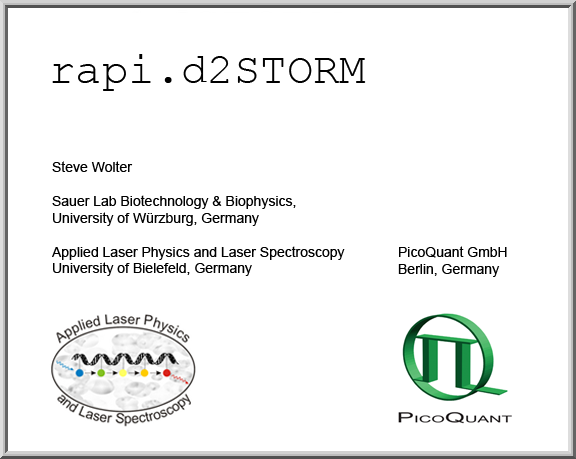
\includegraphics[width=0.205\textwidth]{logo.png} \hspace{10 cm} \includegraphics[width=0.205\textwidth]{klee.jpg}}%\\ Fakult�t f�r Physik}
  \subject {}
  \title {\Large meine LaTeX-Referenz}
  %\author {\sffamily \large vorgelegt von Sven Martin Proppert \vspace {30pt}\\{\small Von der Fakult�t f�r Physik genehmigte}\\Diplom-Arbeit\\{\small zur Erlangung des Grades eines Diplomphysikers.} \vspace {40pt}}
  \author {\sffamily \large vorgelegt von Sven Martin Proppert \vspace {30pt}\\{\small Von der Fakult�t f�r Physik und Astronomie genehmigte}\\Dissertation\\ \vspace {100pt}}
  \date{\today}
  \publishers {\large Gutachter:\\Prof. Dr. rer. nat. Markus Sauer\\Prof. Dr. rer. nat. }
%%end Infos f�r Titlepage
%%end of header



%%your document starts here
\begin{document}
%\sffamily				%%schrift serifenlos

\section{Calibration data}

\subsection{record calibration file}
\par Things needed for recording calibration data\label{tab:reccal}:
\begin{itemize}
	\item rapidSTORM
	\item gnuplot or comparable software
	\item thinly coated Tetraspeck surface
	\item objective piezo (e.g. PIfoc, Physik Instrumente)
	\item appropriate cylindrical lens in detection path
\end{itemize}

Exaple procedure:
\begin{enumerate}
	\item place Tetraspeck surface on microscope
	\item set piezo to remote control
	\item focus on Tetraspeck
	\item make the piezo move around focal plane with a triangular function
	\item record data 
	\item exemplary settings piezo:\\
				low position: 45 $\mu$m\\
				high position: 55 $\mu$m\\
				frequence: 0.02 Hz\\
				function: triangular
	\item exemplary camera settings:\\
				exposure time: 0.02 s
\end{enumerate}

\subsection{get calibration curve}
\begin{enumerate}
	\item start rapidSTORM, load calibration data to the input field (don't forget to check "`Ignore libtiff warnings"' if your data is a tif-file) and switch to expert mode
	\item "`Size of input pixel"': \\
	enter correct pixelsizes for x and y (to get two fields, click the unjoin button)
	\item "`PSF FWHM"': \textbf{remember your input!} \\
	e.g. Alexa 647: 370 nm
	\item "`Amplitude discarding threshold"': \\
	filters rubbish from data. As your Tetraspeck should be very bright, you would want to enter a high value. 2000-5000 will do for a start
	\item "`Fit window radius"': \textbf{remember your input!} \\
	in order to be able to fit widespread PSFs, enter a value considerably higher than  the PSF FHWM. In our example, the value should be around 1100 nm
	\item "`maximum number of iteration steps for spot fitting"':\\
	\item check boxes "`PSF width is free fit parameter"' and "`Store PSF covariance matrix"'
	\item under "`Output options"' go to the "`Expression filter"' menue\\
		\begin{itemize}
			\item "`value to assign to"':\\
			posz
			\item "`Expression to assign from"':\\
			\textit{X} nm/fr * frame\\
			(in this example: 8 nm/fr *frame)
			\item "`Choose new output"':\\
			"`3D PSF width calibration table"'
		\end{itemize}
	\item go to the "`3D PSF width calibration table"' menue\\
		\begin{itemize}
			\item "`FWHM correction for object size"':\\
			Here, you adjust, how much the PSF FWHM of the Tetraspeck differs from the PSF 				FWHM of a fluorophore in your sample. Our value  - still Voodoo - is 25 nm
			\item "`Number of B spline breakpoints"':\\
			10 should be sufficient in most cases. This setting roughly controls the number 			of basic functions used for fitting.
			\end{itemize}
	\item run evaluation
\end{enumerate}

\par rapidSTORM now created some outputs. You should already know the \textit{calibration filename}.txt and the \textit{calibration filename}-raw.txt (and \textit{calibration filename}.png if you saved the picture. The interesting and new output is \textbf{\textit{calibration filename}-sigma-table.txt}. Plot this file with gnuplot or Origin. As you now tried to get an interpolated calibration curve for the whole movie, it is likely that your result will look pretty awful, but that is ok. This is just because the fit routine tried to fit to PSFs which were already too blurred or even showed a first diffraction order. Thus you have to crop the z region that rapidSTORM tries to fit, so first try to estimate, where the fitting is kinda decent. As an exaple, let's assume this is between $z= 2000 nm$ and $z= 6000 nm$.  You now have to do the same as above, but using this extra knowledge. Don't worry, rapidSTORM kept the settings if you didn't close it.

\begin{enumerate}
	\item close old job
	\item go to the "`Expression filter"' tab
		\begin{itemize}
		\item click "`Add expression"'
		\item "`Expression to assign from"' (the blank one):\\
		in this example: posz > 2000 nm \&\& posz < 6000 nm
		\end{itemize}
	\item run evaluation again
	\item have a look at the result
	\item repeat cropping and reevaluating until your calibration curves look smooth and steady
\end{enumerate}

\par You are now ready to calibrate your measurement.

\section{Make 3D image of measurement}

\begin{enumerate}
	\item Load your measurement file in rapidSTORM (make shure, you are still in Expert mode)
	\item "`3D PSF model"'\\
	Choose "`Interpolated 3D"'
	\item Enter the pixelsizes you used for calibration
	\item "`Z calibration file"':\\
	select your final \textit{calibration filename}-sigma-table.txt
	\item adjust "`Amplitude discarding threshold"'
	\item "`Fit window radius"':\\
	\textbf{It is crucial to enter the exact value you used for calibration} (1100 nm in the example)
	\item \textbf{make sure you uncheck "`PSF width is free fit parameter"' and "`Store PSF covariance matrix"'}
	\item go to "`Expression filter"'
		\begin{itemize}
		\item Erase what you entered in the first "`Expression to assign from"'-field (here, 8 nm/fr * frame)
		\item Change the first "`Value to assign to"' from posz to Expression
		\item Erase what you entered in the other "`Expression to assign from"'-field (here, posz > 2000 nm \&\& posz < 6000 nm)
		\item "`Select output to remove"':\\
		3D PSF width calibration table
	\end{itemize}
	\item go to "`Expression filter -> Image Display"'
		\begin{itemize}
		\item "`Save image to"':\\
		Change filetype to .tif. Make sure, the filename differs from the measurements filename. We would suggest to call it 			\textit{filename}\_stack.tif
		\item adjust "`Resolution in x,y,z direction"' fields:\\
		Especially z should get a reasonable value - let's say 50 nm. Else you will most likely run out of memory when saving the stack
		\item Check the "`Make 3D image"' box
		\item you may want to colour-code z position:\\
		"`Colour palette for display"':\\
		Choose "`Vary hue with sample coordinate"'\\
		"`Coordinate to vary hue with"':\\
		"`position in sample space z"'
		\end{itemize}
	\item run evaluation
	\item have a look at your result for example using the fiji image viewer
\end{enumerate}

\par That's it...

%%end is near ;-)
\end{document}


